\chapter{Asking Golf Course Millionaires How They Got Rich}

This episode has no blackboard, but it does have a definite arithmetic. The host opens with a teaser of large exits and seven-figure earnings, then moves through the practical problem of access, and only afterward draws out the rules by which income is held back from consumption, objections are turned into information, capital is assembled, and businesses are scaled. We should therefore read the lecture in the order it gives itself: first the stakes, then the search, then the mechanisms.

\section{Wealth Outcomes Before Method}

The lecture begins with a cold open assembled from later interviews. It does not yet tell us how wealth was made. It tells us only that the game is worth playing: large exits exist, seven-figure years occur, and the people reporting them are scattered across different careers and forms of ownership.

\begin{align}
P_{\text{landscape exit}} &\approx \$42\,\text{million},\\
P_{\text{PostUp exit}} &\approx \$38\,\text{million},\\
I_{\text{seven digits}} &\ge \$10^6.
\end{align}

These are speaker-reported markers, not audited balance-sheet quantities. Their role is motivational. They tell us what kinds of outcomes the later interviews will try to explain. The right question at this stage is not yet ``What is the formula?'' but rather ``What kinds of human and commercial decisions can plausibly sit behind numbers of this size?''

A second feature of the opening is that the outcomes are heterogeneous. One figure comes from selling a landscape supply company after four years. Another comes from the sale of a software company. Others come from peak earning years rather than exits. The lecture is already signaling that there is no single privileged route. What matters is the structure by which value was accumulated and then either paid out annually or realized at sale.

\section{The Access Problem}

Before the lecture can become analytical, it becomes logistical. The team pulls up to Austin Country Club, asks to enter, and is refused unless they are members or residents. This is more than scene-setting. It establishes the governing rhythm of the episode: wealth is not laid out for us in a classroom; it is hidden behind literal and social gates, and the inquiry proceeds by finding openings.

The pivot to the second course matters for the same reason. The speaker says, in effect, that if the first game plan fails, the game plan must change. The gate at the next course is open, but even there the team is aware of attendants, surveillance, and the possibility of being turned away. The lecture's first practical theorem is therefore not about finance at all. It is that access is part of the method. Before we can ask how wealth is made, we must get close enough to ask the question.

That search structure should remain visible in the notes. It prevents the later advice from sounding like an omniscient summary. Each claim comes from an encountered person, at a particular time, under conditions that could easily have prevented the conversation from happening at all.

\section{Means, Mentors, and the First Million}

The first interview cluster gives us a set of personal mechanisms before it gives us a theory of companies. One interviewee reports a peak year of a little over a million dollars and attributes his success to following work he loved, becoming a successful hospital administrator, remaining street smart, and never becoming too full of himself. The sequence is important: passion is not presented as self-expression alone, but as something that can support sustained competence and institutional responsibility.

Then the lecture asks the more interesting financial question: how does one start the path to financial freedom? The answer is brief and severe: live within your means. Immediately after that comes the sharpest piece of arithmetic in the early part of the episode, a mentor's rule to live on what one made five years ago and invest or bank the rest.

If we introduce notation only to clarify the mechanism, we may write
\begin{align}
C_t &\approx Y_{t-5},\\
S_t &= Y_t - C_t,\\
Y_t &= C_t + S_t,
\end{align}
where \(Y_t\) is current income, \(C_t\) is current consumption, and \(S_t\) is the portion that can be banked or invested. The point is not that life obeys an exact law of motion. The point is that by forcing lifestyle to lag income, one converts earnings growth into surplus rather than into immediate inflation of spending.

That is a useful piece of operator arithmetic. It tells us that the first million is not merely a matter of making more. It is a matter of refusing to let current success rewrite one's consumption baseline too quickly.

The next interviewee pushes the lecture from household discipline toward business design. He reports a peak year of roughly \( \$1.5 \) million and says that he currently owns a company built around a golf putting training aid. When asked what advice he would give to someone starting a business this year, the answer is procedural rather than romantic. One needs advice from people who have launched startups successfully, a strong business plan, strong marketing and social media presence, funding in place, and then a people-first operating philosophy.

We may summarize that operating sequence as follows:
\begin{itemize}
\item learn from successful founders,
\item articulate a business plan,
\item build distribution and visibility,
\item secure funding,
\item take care of the people who will take care of the customer.
\end{itemize}

The lecture has now moved from individual restraint to the design of a commercial machine. That widening is crucial. Wealth is not yet reduced to a formula, but its ingredients are becoming more structural.

\section{Intermission as Rhythmic Reset}

At this point the lecture deliberately interrupts itself with the golf challenge involving James and Will. Analytically, little is added here, but rhythmically a great deal is gained. The interruption keeps the episode from flattening into a sequence of compressed aphorisms. It resets attention and makes the return to interviewing feel like a second pass through the same problem, now with sharper questions.

For that reason the intermission should remain visible, though briefly. It is part of the lecture's pacing. It marks the transition from general success talk into more pointed discussions of sales, objections, debt, and eventually capital structure.

\section{Sales, Objections, and Early Investing}

The next important turn is toward sales. One interviewee says he was first a golf professional and then moved into IT sales. When asked for his secret, he gives an answer that is both simple and exact: put yourself in the customer's shoes, build relationships by being personal and real, and listen for the customer's actual challenge. This is not flashy language, but it has a clear operational form.

The key update rule appears when the host asks what happens after a no. The answer is not ``push harder.'' The answer is: find out why. In compact form,
\begin{equation}
\text{No} \longrightarrow \{\text{competition},\ \text{pricing},\ \text{other}\}.
\end{equation}
The refusal is treated as data. A failed sale is turned into a classified objection, and the classification improves the next attempt.

\begin{figure}[h]
\centering
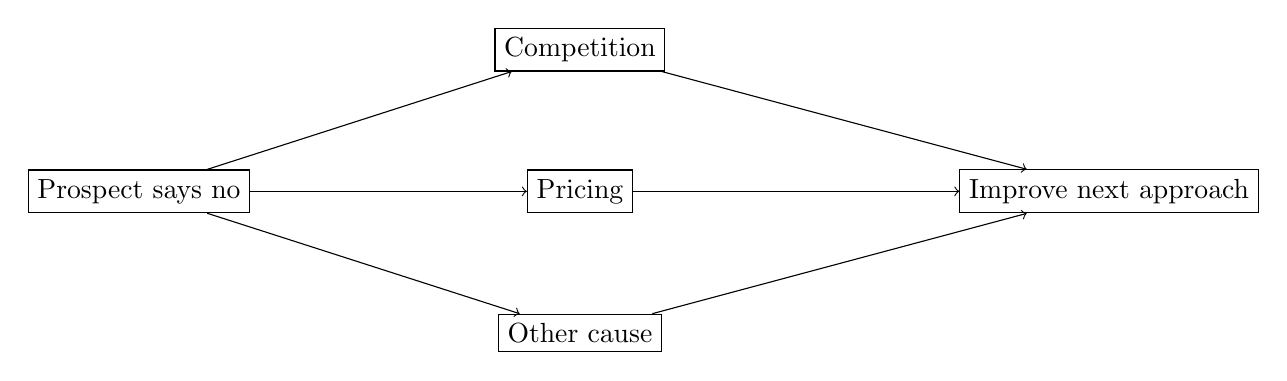
\begin{tikzpicture}[x=2.8cm,y=1.5cm]
\node[draw, rectangle] (no) at (0,0) {Prospect says no};
\node[draw, rectangle] (comp) at (2,1.2) {Competition};
\node[draw, rectangle] (price) at (2,0) {Pricing};
\node[draw, rectangle] (other) at (2,-1.2) {Other cause};
\node[draw, rectangle] (next) at (4.4,0) {Improve next approach};

\draw[->] (no) -- (comp);
\draw[->] (no) -- (price);
\draw[->] (no) -- (other);
\draw[->] (comp) -- (next);
\draw[->] (price) -- (next);
\draw[->] (other) -- (next);
\end{tikzpicture}
\caption{Transcript-derived objection diagnosis. The sale does not end at refusal; the refusal is sorted into a reason and used to improve the next attempt.}
\end{figure}

This is the first place where the lecture sounds unmistakably procedural. It is not merely saying that personal warmth matters. It is saying that sales competence includes a feedback loop.

The advice then swings back to personal finance. We hear the blunt warning to stay out of debt, followed by the joke that divorce is expensive because it has already been experienced as such. Immediately after that, an architect gives a broader comparative claim: he studied with people who did not go to college but became financially free because they made good investments, became business owners, and understood early that money had to be invested. The earlier the investing begins, the better.

So the lecture is now linking three levels of discipline:
\begin{itemize}
\item relational discipline in sales,
\item behavioral discipline in debt avoidance,
\item temporal discipline in starting investment early.
\end{itemize}

The voice of the lecture remains empirical. These are not propositions proved from theory. They are mechanisms reported from practice.

\section{Employment, Ownership, and Company Building}

The next cluster asks a harder question: what sort of career should one want? An older interviewee says that a college degree is important but not imperative. In the same breath he insists that one can start a business in this country, even borrowing on the order of two or three hundred thousand dollars, and adds the striking anecdote that he himself started a company fifty years ago with \( \$67 \) in the bank. The point is not that everyone can reproduce the same path under identical conditions. The point is that the barrier is not framed here as credential alone.

What follows is a moral condition on this claim. The mindset shift needed to become a multimillionaire, he says, is humbleness. One must live correctly, not imagine that everything good was self-manufactured, and not become blinded by one's own success. This part of the lecture should not be ironed into neutral management prose. It belongs to the speaker's own framework.

He then offers an important bifurcation. A person must decide who he is. One route is high-level employment: work for a company like Dell, make a few hundred thousand dollars a year, and enjoy life. Another route is ownership: decide what interests you, then learn from those who have done it before. This is not presented as a universal hierarchy in which ownership always defeats employment. It is presented as a problem of fit.

The software-company interview sharpens that fit into organizational terms. We are told of a career that passed through Sony and Dell and then into software, culminating in the sale of PostUp to Upland Software for about \( \$38 \) million. When asked what scaled the company, the answer is not a slogan about disruption. It is a sequence about people: put good people in places where they will succeed, develop them, get everyone on the same page, and make communication effective.

The mechanism of scale here is therefore not primarily financial. It is coordinative. At larger firms, the speaker says, politics were a major challenge. In a small company one can strip away some of that noise and focus on the customer, the solution, and the product. The lecture is quietly drawing a contrast between scale by bureaucracy and scale by alignment.

\section{Capital, Money Management, and Scale}

After another brief return to the golf match, the lecture resumes with one of its most compressed pieces of financial logic. A later interviewee says that one should fail a lot, find a mentor quickly, and remember that even when reported income rises above a million dollars, the real problem has only begun. More money means more problems if one does not know how to manage the money, keep the money, and grow the money.

That three-stage structure is worth preserving in symbolic shorthand:
\begin{equation}
\text{earn} \longrightarrow \text{keep} \longrightarrow \text{grow}.
\end{equation}
Income by itself is not yet wealth. Retention and compounding sit between the paycheck and durable financial freedom.

The same interviewee adds that younger people often lack personal skills and that those skills matter because much of the available wealth is held by people older than they are. Thus the lecture keeps together two kinds of capital: financial capital and relational capital. It then gives a simple sector observation: medical work is not going away. Here again, the point is not to derive an industry model, but to preserve the concrete institutional claim as it was given.

The final major case then brings the arithmetic of ownership into its clearest form. Another speaker says the advice he would give his younger self is to start his own business. He describes a path through UT, Wharton, KPMG, PWC, and Union Carbide, then says he became disenchanted with corporate America, bought a landscape supply company in New Braunfels, and sold it four years later for approximately \( \$42 \) million. The lecture has now arrived at its sharpest practical question.

\subsection{Question \& Answer}

\paragraph{Question.} Do we need investors in order to start or buy a business?

\paragraph{Answer.} The speaker's answer is no, or at least not necessarily. He says there is a great deal of capital available, that investors can be problematic, and that one can often use SBA-backed borrowing and a relatively small down payment to reach a viable starting position.

Let us formalize only the arithmetic that is actually spoken. If \(d\) denotes the cash-down fraction, then
\begin{align}
d_{3\text{M}} &= \frac{150{,}000}{3{,}000{,}000} = 0.05,\\
d_{1\text{M}} &= \frac{50{,}000}{1{,}000{,}000} = 0.05.
\end{align}

\paragraph{Worked example.}
\begin{enumerate}
\item Define \(d = \dfrac{\text{cash down}}{\text{purchase size}}\).
\item For the first example, the lecture gives \( \$150{,}000 \) down on \( \$3{,}000{,}000 \).
\item Hence \(d = 150{,}000/3{,}000{,}000 = 0.05\), so the down payment is \(5\%\) of the purchase size.
\item For the second example, \( \$50{,}000 \) down on \( \$1{,}000{,}000 \) gives the same fraction:
\(50{,}000/1{,}000{,}000 = 0.05\).
\end{enumerate}

These are examples, not universal lending laws. Still, they matter because they make the speaker's claim concrete. The lecture is saying that the initial equity requirement for entering ownership may be much smaller than many young listeners imagine.

Once the capital question is answered, the lecture closes the loop by returning to scale. The same speaker says the biggest thing he did was believe in growth. The details are notably operational:
\begin{itemize}
\item buy more trucks when others doubt the purchase,
\item hire more people when the team is stressed,
\item buy better equipment,
\item outsource service work so managerial attention can stay on the business itself.
\end{itemize}

We should notice what this means. Scale is not described here as a miracle of branding. It is described as a chain of capacity decisions. If each new truck makes more money, if hiring removes strain, and if outsourcing frees the operator to think at the level of the business rather than the level of daily service work, then scale becomes a disciplined widening of bottlenecks rather than an act of blind optimism.

\section{Summary}

The lecture begins with outcomes, but it earns those outcomes only gradually. First comes the search for access. Then come rules of personal conduct: passion, humility, street smarts, living within one's means, and allowing spending to lag income. Then come rules of commercial conduct: diagnose objections, invest early, decide honestly between employment and ownership, place good people well, and keep them aligned. Finally comes the most concrete arithmetic of the episode: capital may be available with less cash down than the novice expects, investors may not be the only path, and scale often comes from repeated capacity decisions rather than from a single stroke of genius.

That is the chapter's real mathematical payload. It is not advanced finance. It is operator arithmetic: how earnings turn into surplus, how refusal turns into information, how down payments turn into control, and how growth turns into a sequence of tractable decisions.